\documentclass[aspectratio=169,11pt]{beamer}

\usepackage[T1]{fontenc}
\usepackage[utf8]{inputenc}
\usepackage{lmodern}
\usepackage{graphicx}
\usepackage{booktabs}
\usepackage{amsmath}
\usepackage{array}
\usepackage{xcolor}
\usepackage{tikz}
\usepackage{hyperref}

% ---------------------------------------------------------------------------
% Audit-friendly metadata: replace these placeholders before the presentation.
% ---------------------------------------------------------------------------
\newcommand{\PresenterName}{YOUR NAME}
\newcommand{\StudentID}{YOUR STUDENT ID}
\newcommand{\TeamMembers}{YOUR TEAM MEMBERS}
\newcommand{\CourseName}{AIAA3800 --- Human-Centered Artificial Intelligence}
\newcommand{\PresentationDate}{Monday, 27 July 2026}

% ---------------------------------------------------------------------------
% Visual system
% ---------------------------------------------------------------------------
\definecolor{Navy}{HTML}{112B52}
\definecolor{Blue}{HTML}{1F5FBF}
\definecolor{Teal}{HTML}{148777}
\definecolor{Orange}{HTML}{E96B2C}
\definecolor{Purple}{HTML}{7650B5}
\definecolor{Ink}{HTML}{172033}
\definecolor{Muted}{HTML}{5C667A}
\definecolor{PaleBlue}{HTML}{EEF4FC}
\definecolor{PaleTeal}{HTML}{EDF8F5}
\definecolor{PaleOrange}{HTML}{FFF3EC}
\definecolor{Line}{HTML}{D6DCE7}

\setbeamercolor{normal text}{fg=Ink,bg=white}
\setbeamercolor{frametitle}{fg=Navy,bg=white}
\setbeamercolor{structure}{fg=Blue}
\setbeamercolor{alerted text}{fg=Orange}
\setbeamercolor{footline}{fg=Muted,bg=white}

\setbeamerfont{title}{series=\bfseries,size=\fontsize{42}{46}}
\setbeamerfont{subtitle}{size=\fontsize{18}{22}}
\setbeamerfont{frametitle}{series=\bfseries,size=\fontsize{24}{28}}
\setbeamerfont{normal text}{size=\fontsize{14}{18}}
\setbeamerfont{footline}{size=\fontsize{9}{11}}
\setbeamerfont{caption}{size=\fontsize{10}{12}}

\setbeamertemplate{navigation symbols}{}
\setbeamertemplate{itemize item}{\color{Teal}\raisebox{0.15ex}{\rule{0.75ex}{0.75ex}}}
\setbeamertemplate{itemize subitem}{\color{Blue}\raisebox{0.15ex}{\rule{0.55ex}{0.55ex}}}
\setbeamersize{text margin left=0.72cm,text margin right=0.72cm}
\setlength{\leftmargini}{1.25em}

\setbeamertemplate{frametitle}{%
  \nointerlineskip
  \vspace{0.25cm}
  \begin{beamercolorbox}[wd=\paperwidth,leftskip=0.72cm,rightskip=0.72cm,sep=0pt]{frametitle}
    \usebeamerfont{frametitle}\insertframetitle
  \end{beamercolorbox}
  \vspace{0.12cm}
  {\color{Line}\rule{\textwidth}{0.6pt}}
}

\setbeamertemplate{footline}{%
  \leavevmode
  \hbox{%
    \begin{beamercolorbox}[wd=.76\paperwidth,ht=0.32cm,dp=0.16cm,leftskip=0.72cm]{footline}
      \usebeamerfont{footline}\CourseName
    \end{beamercolorbox}%
    \begin{beamercolorbox}[wd=.20\paperwidth,ht=0.32cm,dp=0.16cm,rightskip=0.72cm plus1fil]{footline}
      \usebeamerfont{footline}\insertframenumber
    \end{beamercolorbox}%
  }
}

\newcommand{\bigmetric}[3]{%
  \begin{minipage}[t]{0.45\linewidth}
    {\color{#1}\bfseries\fontsize{38}{41}\selectfont #2\par}
    \vspace{0.06cm}
    {\fontsize{15}{19}\selectfont #3\par}
  \end{minipage}
}

\newcommand{\sourcefooter}[1]{%
  \vfill
  {\color{Muted}\fontsize{8.5}{10}\selectfont Source: #1\par}
}

\title{EEG-to-Image Retrieval}
\subtitle{Brain--vision alignment with lightweight visual adaptation}
\author{\PresenterName\quad|\quad \StudentID}
\institute{\CourseName\\[0.08cm]\TeamMembers}
\date{\PresentationDate}

\begin{document}

% ---------------------------------------------------------------------------
\begin{frame}[plain]
% [Sources]
% - Repository README_ZH.md (project title, course context, and main method).
  \vspace{0.42cm}
  {\color{Teal}\bfseries\fontsize{14}{17}\selectfont HUMAN-CENTERED AI COURSE PROJECT\par}
  \vspace{0.30cm}
  {\color{Navy}\bfseries\fontsize{42}{46}\selectfont EEG-to-Image\\Retrieval\par}
  \vspace{0.18cm}
  {\color{Muted}\fontsize{18}{22}\selectfont Brain--vision alignment with lightweight visual adaptation\par}
  \vfill
  {\fontsize{12}{15}\selectfont
    \textbf{\PresenterName}\quad \StudentID\\[0.08cm]
    \TeamMembers\\[0.10cm]
    \CourseName\quad|\quad\PresentationDate
  }
  \vspace{0.35cm}
\end{frame}

% Speaker note: Open with the question, not the model. The task is to retrieve a
% viewed image from a gallery using non-invasive EEG.

% ---------------------------------------------------------------------------
\begin{frame}{Start with the human question}
% [Sources]
% - Gifford et al. (2022), THINGS-EEG dataset paper.
% - Repository README_ZH.md, "Limitations and responsible use".
  \vspace{0.35cm}
  {\color{Navy}\bfseries\fontsize{22}{27}\selectfont
    Can a non-invasive brain signal retrieve what a person has just seen?
  \par}
  \vspace{0.55cm}

  \begin{columns}[T,onlytextwidth]
    \column{0.31\textwidth}
      {\color{Blue}\bfseries\fontsize{20}{24}\selectfont Useful\par}
      \vspace{0.12cm}
      {\fontsize{14}{18}\selectfont Connect neural activity to interpretable visual semantics.}

    \column{0.31\textwidth}
      {\color{Teal}\bfseries\fontsize{20}{24}\selectfont Constrained\par}
      \vspace{0.12cm}
      {\fontsize{14}{18}\selectfont Work within noisy, subject-specific EEG rather than claiming mind reading.}

    \column{0.31\textwidth}
      {\color{Orange}\bfseries\fontsize{20}{24}\selectfont Responsible\par}
      \vspace{0.12cm}
      {\fontsize{14}{18}\selectfont Treat consent, privacy, and non-clinical use as design requirements.}
  \end{columns}

  \sourcefooter{THINGS-EEG2; project responsible-use statement.}
\end{frame}

% Speaker note: Emphasize that the system predicts among known gallery images.
% It is not a clinical system and does not reconstruct arbitrary thoughts.

% ---------------------------------------------------------------------------
\begin{frame}{A difficult task with a precise metric}
% [Sources]
% - Repository README_ZH.md, "Original project experimental configuration".
% - Gifford et al. (2022), THINGS-EEG2.
  \vspace{0.08cm}
  \begin{columns}[T,onlytextwidth]
    \column{0.55\textwidth}
      {\color{Navy}\bfseries\fontsize{20}{24}\selectfont Subject-wise EEG decoding\par}
      \vspace{0.25cm}
      \begin{itemize}
        \item 10 participants from THINGS-EEG2
        \item 17 posterior EEG channels
        \item Repeated trials averaged within each stimulus
        \item 512-dimensional shared embedding space
      \end{itemize}

    \column{0.39\textwidth}
      {\color{Orange}\bfseries\fontsize{34}{38}\selectfont 200-way\par}
      {\fontsize{16}{20}\selectfont zero-shot image retrieval\par}
      \vspace{0.48cm}
      {\color{Muted}\fontsize{14}{18}\selectfont Chance performance\par}
      \vspace{0.08cm}
      {\color{Navy}\bfseries\fontsize{21}{25}\selectfont 0.5\% Top-1\par}
      {\color{Navy}\bfseries\fontsize{21}{25}\selectfont 2.5\% Top-5\par}
  \end{columns}

  \vspace{0.08cm}
  {\color{Teal}\rule{\textwidth}{2.4pt}}
  \vspace{0.08cm}
  {\fontsize{13}{16}\selectfont
    Success: rank the exact held-out image above 199 alternatives.
  \par}
  \sourcefooter{Project protocol: independent cosine-similarity ranking for each EEG query.}
\end{frame}

% Speaker note: Explain why the chance baseline is low and why exact-image
% retrieval is stricter than category-template recognition.

% ---------------------------------------------------------------------------
\begin{frame}[plain]
% [Sources]
% - Project-authored visual: asserts/Architecture.png.
  \centering
  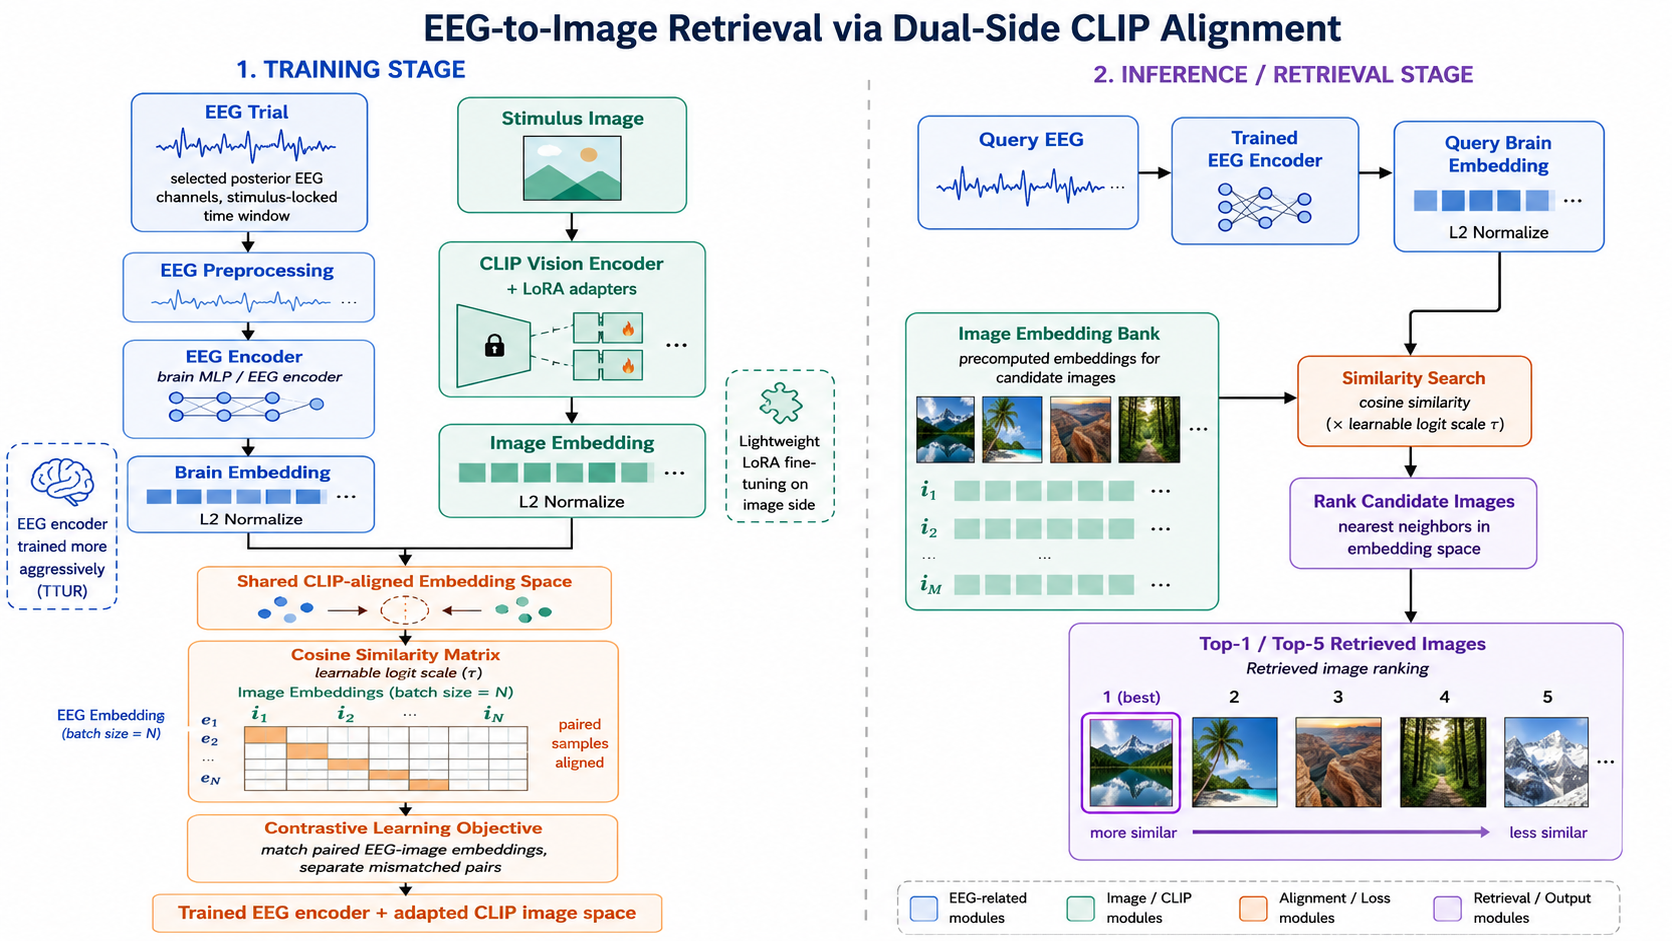
\includegraphics[width=\textwidth,height=0.96\paperheight,keepaspectratio]{assets/Architecture.png}
\end{frame}

% Speaker note: Walk left-to-right. Training aligns EEG and image embeddings;
% inference freezes the trained system and ranks a precomputed image bank.

% ---------------------------------------------------------------------------
\begin{frame}{LoRA and TTUR align both modalities}
% [Sources]
% - Repository README_ZH.md, "Method" and experimental configuration.
% - Hu et al. (2022), LoRA.
  \vspace{0.22cm}
  \begin{columns}[T,onlytextwidth]
    \column{0.48\textwidth}
      {\color{Blue}\bfseries\fontsize{20}{24}\selectfont Brain branch\par}
      \vspace{0.12cm}
      {\fontsize{14}{18}\selectfont
        A residual MLP maps posterior-channel EEG into the CLIP-aligned
        512-D space.
      \par}
      \vspace{0.38cm}
      {\color{Navy}\bfseries\fontsize{18}{22}\selectfont Faster adaptation\par}
      {\fontsize{15}{19}\selectfont $\eta_{\text{brain}} = 5\times10^{-4}$}

    \column{0.48\textwidth}
      {\color{Teal}\bfseries\fontsize{20}{24}\selectfont Visual branch\par}
      \vspace{0.12cm}
      {\fontsize{14}{18}\selectfont
        Rank-32 LoRA updates CLIP ViT-B/32 without fully retraining the
        visual backbone.
      \par}
      \vspace{0.38cm}
      {\color{Navy}\bfseries\fontsize{18}{22}\selectfont Slower coordination\par}
      {\fontsize{15}{19}\selectfont $\eta_{\text{vision}} = 5\times10^{-5}$}
  \end{columns}

  \vspace{0.16cm}
  \begin{center}
    {\color{Orange}\bfseries\fontsize{15}{19}\selectfont
      Contrastive alignment joins paired EEG and image embeddings.
    \par}
  \end{center}
  \sourcefooter{Project configuration: CLIP ViT-B/32, LoRA rank 32, TTUR-style learning rates.}
\end{frame}

% Speaker note: TTUR is the key intuition: the noisy brain encoder learns
% aggressively, while the pretrained visual space moves conservatively.

% ---------------------------------------------------------------------------
\begin{frame}{Evaluation designed to resist optimism}
% [Sources]
% - Repository README_ZH.md, "Reproducibility policy".
% - experiments/samga_lora/AUDIT_LOG.md.
  \vspace{0.22cm}
  \begin{columns}[T,onlytextwidth]
    \column{0.39\textwidth}
      {\color{Navy}\bfseries\fontsize{36}{40}\selectfont 50\par}
      {\fontsize{17}{21}\selectfont independently trained models\par}
      \vspace{0.18cm}
      {\color{Muted}\fontsize{14}{18}\selectfont
        10 subjects $\times$ 5 seeds
      \par}

    \column{0.57\textwidth}
      \begin{enumerate}
        \item[\color{Blue}\textbf{01}] Fixed final checkpoint at epoch 25
        \vspace{0.18cm}
        \item[\color{Teal}\textbf{02}] One independent ranking per query
        \vspace{0.18cm}
        \item[\color{Orange}\textbf{03}] Reloaded checkpoints reproduce metrics and predictions
        \vspace{0.18cm}
        \item[\color{Purple}\textbf{04}] No Hungarian assignment in standard results
      \end{enumerate}
  \end{columns}

  \vspace{0.28cm}
  {\color{Line}\rule{\textwidth}{0.8pt}}
  \vspace{0.14cm}
  {\fontsize{14}{18}\selectfont
    The test set reports performance; it does not choose the checkpoint.
  \par}
  \sourcefooter{Five-seed protocol and artifact reload checks documented in the repository.}
\end{frame}

% Speaker note: This slide is part of the contribution. Strong numbers are only
% useful when their selection and aggregation rules are explicit.

% ---------------------------------------------------------------------------
\begin{frame}{The viewed image is retrieved reliably}
% [Sources]
% - Repository README_ZH.md, verified five-seed ten-subject results.
  \vspace{0.12cm}
  \begin{center}
    \bigmetric{Blue}{86.66\%}{Top-1 accuracy\\{\color{Muted}$\pm$ 0.69 points across seeds}}
    \hfill
    \bigmetric{Teal}{98.38\%}{Top-5 accuracy\\{\color{Muted}$\pm$ 0.14 points across seeds}}
  \end{center}

  \vspace{0.10cm}
  \begin{center}
    {\fontsize{15}{19}\selectfont
      \textbf{8,666 / 10,000} Top-1 decisions and
      \textbf{9,838 / 10,000} Top-5 decisions were correct.
    \par}
    \vspace{0.16cm}
    {\color{Orange}\bfseries\fontsize{18}{22}\selectfont
      Top-1 performance is more than 170$\times$ chance.
    \par}
  \end{center}

  \sourcefooter{Five seed-level macro averages; 200 queries per subject and seed.}
\end{frame}

% Speaker note: Avoid calling 10,000 decisions independent samples; the same
% held-out stimuli are evaluated across five seeds.

% ---------------------------------------------------------------------------
\begin{frame}{Visual LoRA helps in a controlled test}
% [Sources]
% - experiments/samga_lora/README.md, confirmatory result.
% - docs/protocols/SAMGA_LORA_EXPERIMENT_PLAN_ZH.md.
  \vspace{0.10cm}
  {\fontsize{14}{18}\selectfont
    All training factors are matched except frozen versus LoRA-adapted CLIP.
  \par}
  \vspace{0.18cm}

  \begin{center}
  \renewcommand{\arraystretch}{1.34}
  \begin{tabular}{>{\raggedright\arraybackslash}p{5.7cm}cc}
    \toprule
    \textbf{Controlled arm} & \textbf{Top-1} & \textbf{Top-5}\\
    \midrule
    Frozen CLIP SAMGA & 76.17\% & 95.79\%\\
    SAMGA + visual LoRA/TTUR & \textbf{\color{Teal}82.68\%} & \textbf{\color{Teal}97.67\%}\\
    \bottomrule
  \end{tabular}
  \end{center}

  \vspace{0.18cm}
  \begin{center}
    {\color{Orange}\bfseries\fontsize{22}{26}\selectfont +6.51 Top-1 points\par}
    {\color{Muted}\fontsize{13}{17}\selectfont
      95\% CI: [+5.22, +7.69] \quad|\quad 48 of 50 paired cells improved
    \par}
  \end{center}
  \sourcefooter{Pre-registered paired comparison; 10,000 two-way subject/seed bootstrap resamples.}
\end{frame}

% Speaker note: This identifies the intervention effect within a CLIP-controlled
% setting. It is not an exact reproduction of SAMGA's InternViT paper result.

% ---------------------------------------------------------------------------
\begin{frame}{Accuracy is not enough}
% [Sources]
% - Repository README_ZH.md, "Limitations and responsible use".
  \vspace{0.22cm}
  \begin{columns}[T,onlytextwidth]
    \column{0.48\textwidth}
      {\color{Blue}\bfseries\fontsize{20}{24}\selectfont What the evidence supports\par}
      \vspace{0.18cm}
      \begin{itemize}
        \item Within-subject, 200-way retrieval
        \item Averaged repeated EEG trials
        \item Stable performance across five seeds
      \end{itemize}

    \column{0.48\textwidth}
      {\color{Orange}\bfseries\fontsize{20}{24}\selectfont What it does not support\par}
      \vspace{0.18cm}
      \begin{itemize}
        \item Cross-subject generalization
        \item Single-trial mind reading
        \item Clinical or diagnostic interpretation
      \end{itemize}
  \end{columns}

  \vspace{0.20cm}
  {\color{Teal}\rule{\textwidth}{2.4pt}}
  \vspace{0.14cm}
  {\fontsize{13}{16}\selectfont
    Consent, privacy, licensing, and restrained claims are part of system quality.
  \par}
  \sourcefooter{Project limitation and responsible-use policy.}
\end{frame}

% Speaker note: Human-centered evaluation includes the boundaries of use, not
% just predictive accuracy.

% ---------------------------------------------------------------------------
\begin{frame}{One strong result, one honest frontier}
% [Sources]
% - Repository README_ZH.md and docs/brain_rw_progress.md.
  \vspace{0.12cm}
  {\color{Navy}\bfseries\fontsize{19}{23}\selectfont
    EEG can be aligned with visual semantics for reliable image retrieval.
  \par}
  \vspace{0.46cm}

  \begin{columns}[T,onlytextwidth]
    \column{0.48\textwidth}
      {\color{Teal}\bfseries\fontsize{20}{24}\selectfont Established\par}
      \vspace{0.14cm}
      {\fontsize{13}{16}\selectfont
        Validated retrieval: dual-side alignment, LoRA/TTUR, five seeds,
        and controlled attribution.
      \par}

    \column{0.48\textwidth}
      {\color{Purple}\bfseries\fontsize{20}{24}\selectfont Next frontier\par}
      \vspace{0.14cm}
      {\fontsize{13}{16}\selectfont
        Retrieval-augmented reconstruction remains exploratory until its
        benefit is reproducible.
      \par}
  \end{columns}

  \vspace{0.22cm}
  \begin{center}
    {\color{Orange}\bfseries\fontsize{15}{19}\selectfont
      Performance, uncertainty, and responsible boundaries belong in the same result.
    \par}
  \end{center}
\end{frame}

% Speaker note: Close by resolving the opening question and naming the next
% scientific step without overselling reconstruction.

% ---------------------------------------------------------------------------
\appendix
\begin{frame}{Selected references}
% [Sources]
% - All entries below are also listed in repository README_ZH.md.
  \vspace{0.10cm}
  {\fontsize{10.5}{13.5}\selectfont
  \begin{thebibliography}{9}
    \bibitem{things}
    Gifford et al. (2022).
    \newblock A large and rich EEG dataset for modeling human visual object recognition.
    \newblock \emph{NeuroImage}.

    \bibitem{atm}
    Li et al. (2024).
    \newblock Visual decoding and reconstruction via EEG embeddings with guided diffusion.
    \newblock \emph{NeurIPS}.

    \bibitem{lora}
    Hu et al. (2022).
    \newblock LoRA: Low-rank adaptation of large language models.
    \newblock \emph{ICLR}.

    \bibitem{samga}
    Jiang et al. (2026).
    \newblock Subject-aware multi-granularity alignment for zero-shot EEG-to-image retrieval.
    \newblock \emph{arXiv preprint}.

  \end{thebibliography}
  }
\end{frame}

\end{document}
